\chapter{New Coordination Geometries for \texorpdfstring{\ce{Re^I}}{Rhenium (I)}}\label{chap.newchem}
\markright{New Coordination Geometries for \texorpdfstring{\ce{Re^I}}{Rhenium (I)}} % new right header
%======================================================================
\section{Introduction}
%======================================================================

As mentioned in the introduction, \ce{Re^I} compounds have been typically bidentate (\ce{$\kappa$^2}) compounds, even when using a potentially terdentate (\ce{$\kappa$^3}) ligand such as bis(imino)pyridine or terpyridine (refer to \autoref{fig.terdentateligands}). The chemistry of this rhenium $\alpha$-imino complex has been extensively invesigated, with over 1700 references appearing in a structure search for that metal-ligand motif. The ejection of an additional carbonyl and the chelation of the pendant arm of the ligand was attempted to extend the conjugated $\pi$ system of the ligand and its interaction with the metal centre. This was first demonstrated by prior work in our group for the bis(imino)pyridine ligand\autocite{jurca2013}. 

%======================================================================
\section{Synthesis of Bidentate and Terdentate \texorpdfstring{\ce{Re^I}}{Rhenium (I)} Complexes}
%======================================================================

Similar to the prior work, synthesis began with the production of the bidentate complex \ce{$\kappa$^2(terpy)Re(CO)3X} (X = Cl, Br) by coordination of 2,2':6',2''-terpyridine with a \ce{Re(CO)5X} starting material in dry toluene at reflux for 4 hours, as shown in \autoref{scheme.bidentate}. A bright yellow powder precipitated from solution and was collected by filtration, washed with cold hexanes, and dried \textit{in vacuo} to a good yield of \textbf{2.1} and \textbf{2.3} respectively.\footnote{Experimental details for all compounds can be seen in \autoref{chap.exp} \nameref{chap.exp}} These bidentate compounds were characterized fully and used without further purification to produce \ce{$\kappa$^3(terpy)Re(CO)2X} (X = Cl, Br) via thermolysis, as well as for anion exchange reactions. 

\begin{scheme}[!htb]
 \begin{center}
  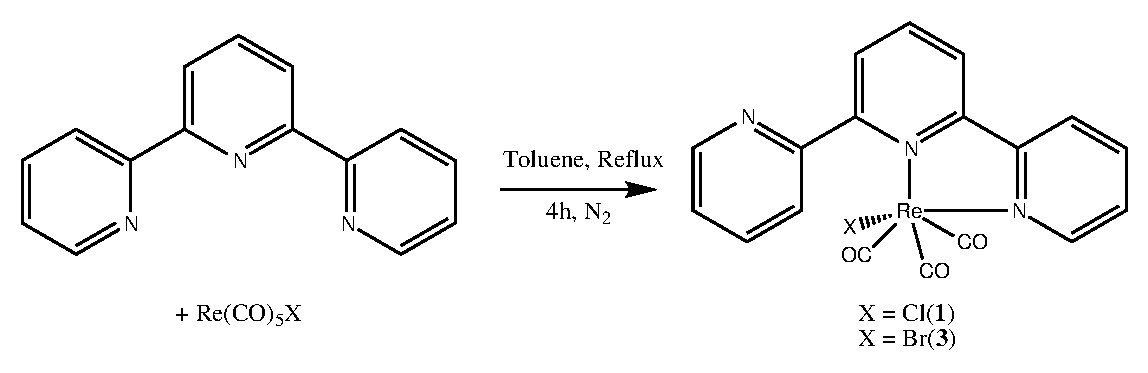
\includegraphics[clip=true, width=140mm, keepaspectratio]{images/bidentate.eps}
 \end{center}
\caption[Synthesis of \textbf{2.1} and \textbf{2.3}]{Synthesis of \textbf{2.1} and \textbf{2.3} from \ce{Re(CO)5X} and 2,2':6',2''-terpyridine}
\label{scheme.bidentate}
\end{scheme} 

Conversion of compounds \textbf{2.1} and \textbf{2.3} to the $\kappa^3$ moiety required the release of \ce{CO} and the subsequent coordination of the free pendant arm. Prior work had identified the thermal lability of the carbonyl, based on a method first described by Buckingham with a osmium complexes\autocite{buckingham1964}. In this method, a ceramic sample boat was placed in a tube furnace at elevated temperature, under a flowing atmosphere of \ce{N2}. After some time, the sample is removed and collected at nearly quantitative yield. Determination of the appropriate thermolysis temperature was performed by \gls{ac.tga} of the sample. A loss of 6-8 \% of starting mass from the sample is consistent with the loss of one carbonyl group from the complex. Results of \gls{ac.tga} on \textbf{2.1} and \textbf{2.3} is shown in \autoref{fig.tga}.

\begin{figure}[!htbp]
 \begin{center}
  \includegraphics[clip=true, width=140mm]{images/tga.eps}
 \end{center}
\caption[Results of \glsentrytext{ac.tga} analysis on \textbf{2.1} and \textbf{2.3}]{Results of \glsentrytext{ac.tga} analysis on \textbf{2.1} and \textbf{2.3}}
\label{fig.tga}
\end{figure} 

The onset of mass loss in the \gls{ac.tga} of \textbf{2.1}, and the onset of the main mass loss in the \gls{ac.tga} of \textbf{2.3} were chosen to identify a thermolysis temperature for each sample. For \textbf{2.1}, thermolysis was performed at 240~$^\circ$C, and for \textbf{2.3} thermolysis was performed at 260~$^\circ$C, yielding \textbf{2.2} and \textbf{2.4} respectively, at quantitative yields, by the pathway in \autoref{scheme.terdentate}.

\begin{scheme}[!htb]
 \begin{center}
  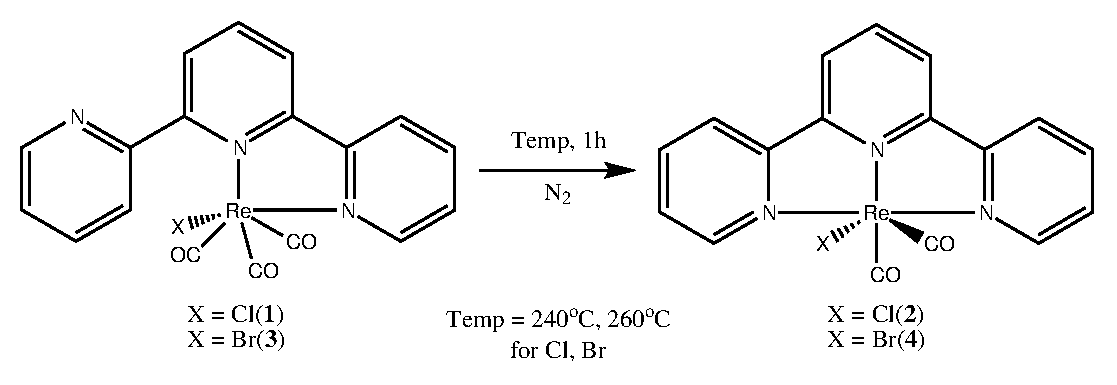
\includegraphics[clip=true, width=140mm, keepaspectratio]{images/thermolysis.eps}
 \end{center}
\caption[Synthesis of \textbf{2.2} and \textbf{2.4}]{Synthesis of \textbf{2.2} and \textbf{2.4} by thermolysis of \textbf{2.1} or \textbf{2.3}, respectively}
\label{scheme.terdentate}
\end{scheme} 

\begin{scheme}[!htbp]
 \begin{center}
  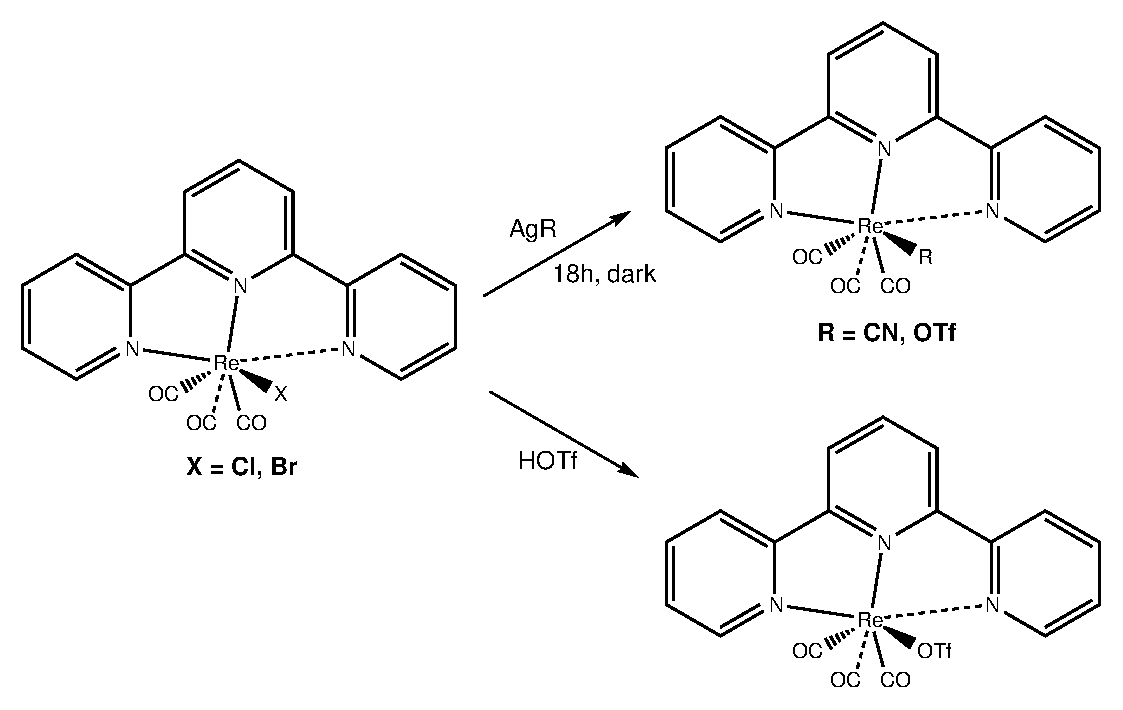
\includegraphics[clip=true, keepaspectratio, width=120mm]{images/anionscheme.eps}
 \end{center}
\caption[Anion exchange pathways]{Anion exchange pathways to synthesize \textbf{2.5} - \textbf{2.8}}
\label{scheme.anion}
\end{scheme}

Further reactions were carried out on the above products to yield triflate and cyano complexes in bidentate and terdentate geometries. These anion exchange reactions were performed by the addition of the silver salt to the chloride products \textbf{2.1} or \textbf{2.2}, to precipitate \ce{AgCl}, leaving \ce{$\kappa$^2(terpy)Re(CO)3CN} (\textbf{2.5}), \ce{$\kappa$^3(terpy)Re(CO)2CN} (\textbf{2.6}), \ce{$\kappa$^2(terpy)Re(CO)3OTf} (\textbf{2.7a}) and \ce{$\kappa$^3(terpy)Re(CO)2OTf} (\textbf{2.8a}), as shown in \autoref{scheme.anion}. Reaction with the bromide products proceeds with similar results. As the Ag anion exchange reactions result in only moderate yields, \textbf{2.7b} was synthesized by the direct addition of neat triflic acid (\ce{CF3SO3H}) to \textbf{2.1}. \ce{HCl} was released, the solutions were quenched by addition of dilute aqueous \ce{NaCO3}, and product was collected via separation into chloroform, again at moderate yield. 

%A pseudo-terdentate complex was targeted to compare \ce{CO2} photoreduction performace with the previously prepared catalysts. Typical \ce{[L2L$'$Re(CO)_n]+} (n = 2, 3) targets exchange the halide for a neutral phosphine or imine type ligand, resulting in a cationic species with weakly coordinated anion (typically \ce{BF4-}, \ce{OTf-}, \ce{BArF-} or other anion)\todo{ref}. Instead, we targeted the \ce{L2L$'$Re(CO)2Cl} (L = bipy, L$'$ = 4-\textit{t}-butylpyridine) compound (\textbf{9}) via two similar methods (\autoref{scheme.pseudo}).

%\missingfigure{anion exchange reaction schemes}
%\begin{scheme}[!htbp]
% \begin{center}
%  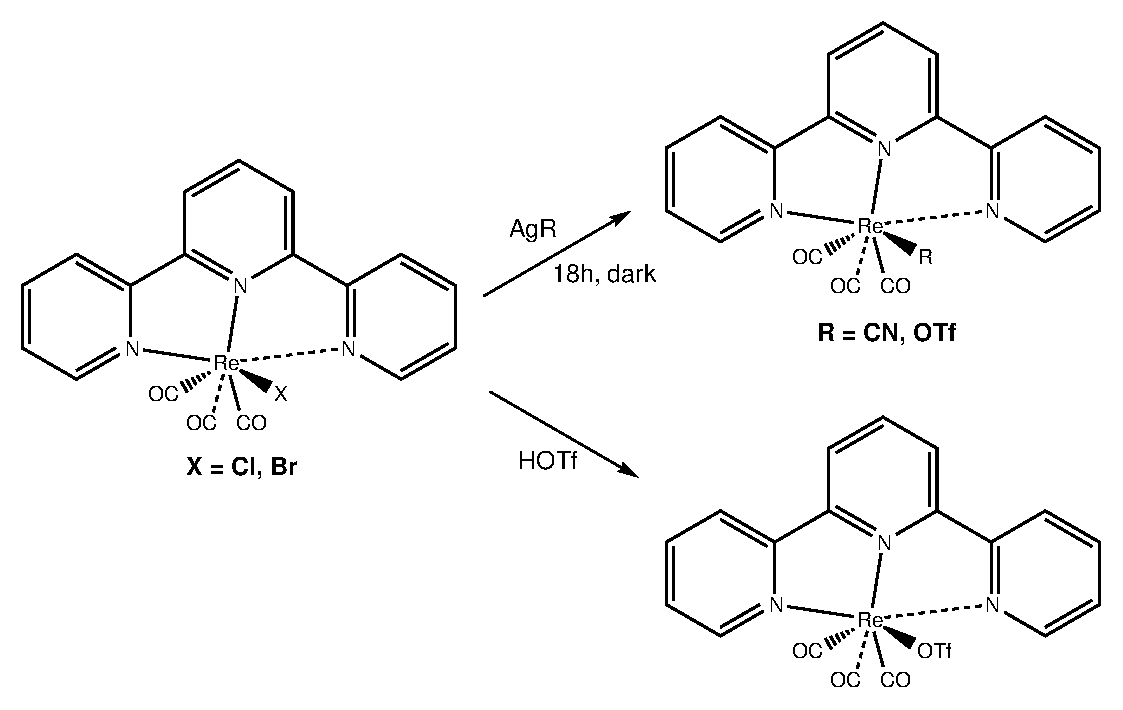
\includegraphics[clip=true]{images/anionscheme.eps}
% \end{center}
%\caption[Synthesis of pseudo-terdentate]{Synthesis of \ce{L2L$'$Re(CO)2Cl} (L = bipy, L$'$ = 4-\textit{t}-butylpyridine) (\textbf{9})}
%\label{scheme.pseudo}
%\end{scheme} %

%======================================================================
\section{Characterization}
%======================================================================

Full characterization was performed, including \Gls{ac.nmr} analysis, x-ray crystallography, elemental analysis, as well as UV-Vis and IR spectroscopy. Computational \gls{ac.dft} methods were used to solve the geometries, and \gls{ac.tddft} was performed to predict UV-Vis spectra and identify electronic transitions. 

%----------------------------------------------------------------------
\subsection{NMR Analysis}
%----------------------------------------------------------------------

Proton \gls{ac.nmr} was performed on each of the samples. Each sample was dissolved completely in deuterated acetonitrile (\ce{CD3CN}) and analysis was performed on a Bruker AVANCE 400 MHz spectrometer. Data was processed from the FID signal via the TopSpin program, and spectra were analyzed using ACD NMR Processor v12.0. 

Detailed peak analysis comparing bidentate samples \textbf{2.1}, \textbf{2.3}, \textbf{2.5}, and \textbf{2.7} (\autoref{fig.bid4nmr}) or terdentate \textbf{2.2}, \textbf{2.4}, \textbf{2.6}, and \textbf{2.8} (\autoref{fig.ter4nmr}) show little difference between samples. This is due to the distance between the anion and any protons on the ligand. While anions with different $\sigma$-donor strength marginally impact the metal-ligand interactions, these have only small effect on the location of peaks, shifting between samples by typically less than 0.1 ppm. As is shown in \autoref{fig.bid4nmr}, the characteristic shape of each spectra remains constant, only exact peak locations and some peak order varies with anion choice. 


\begin{figure}[!htb]
 \begin{center}
  \includegraphics[clip=true, width=\textwidth, keepaspectratio]{images/allbidnmr.eps}
 \end{center}
\caption[The aromatic region of the \texorpdfstring{\ce{^1H}}{1H} \glsentrytext{ac.nmr} spectra of the four bidentate compounds]{The aromatic region of the \texorpdfstring{\ce{^1H}}{1H} \glsentrytext{ac.nmr} spectra for compounds \textbf{2.1} (blue), \textbf{2.3} (green), \textbf{2.5} (red) and \textbf{2.7} (purple)}
\label{fig.bid4nmr}
\end{figure} 

The characteristic feature in the \gls{ac.nmr} spectra after the transformation from bidentate to terdentate (e.g. sample \textbf{2.1} to \textbf{2.2}) is the reduction in the total number of the signals in the aromatic region (between 7 and 9 ppm). This simplification is due to the increased symmetrization of the ligand, while the \ce{$\kappa$^2}-bidentate ligand has a freely rotating pendant group. Prior work in literature\autocite{abel1993} and in our group\autocite{jurca2012} shows the temperature dependence of the rate of rotation of this pendant arm for various ligand species. However, the \ce{$\kappa$^3}-terdentate species has no free groups, the rigid geometry and higher order symmetry results in the simpler \gls{ac.nmr} spectrum.

\begin{figure}[!htb]
 \begin{center}
  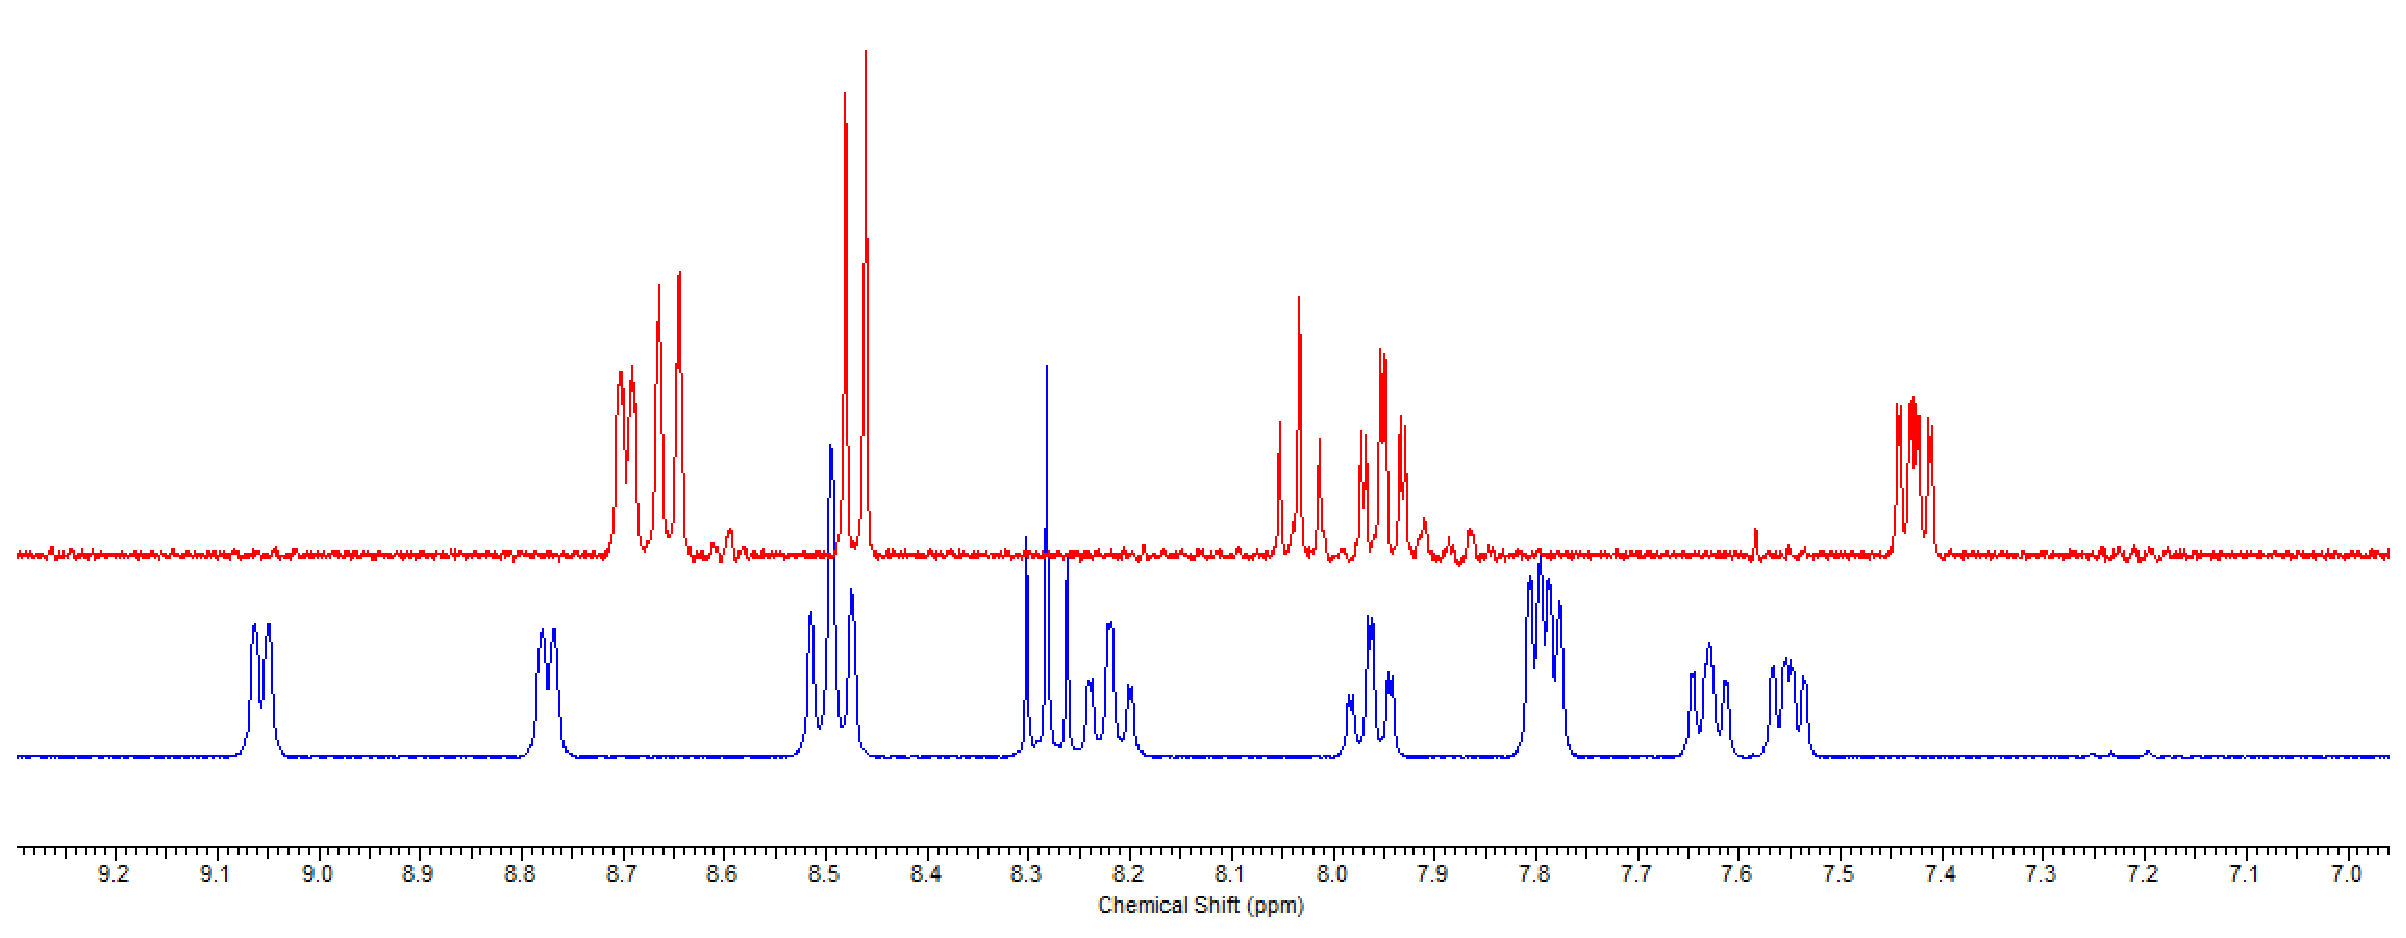
\includegraphics[clip=true, width=\textwidth, keepaspectratio]{images/bidternmr.eps}
 \end{center}
\caption[The aromatic region of the \texorpdfstring{\ce{^1H}}{1H} \glsentrytext{ac.nmr} spectra showing bidentate - terdentate conversion]{The aromatic region of the \texorpdfstring{\ce{^1H}}{1H} \glsentrytext{ac.nmr} spectra for compounds \textbf{2.1} (blue) and \textbf{2.2} (red), showing the simplification of the spectra upon the conversion from bidentate to terdentate}
\label{fig.bidtoter}
\end{figure} 

\begin{figure}[!htb]
 \begin{center}
  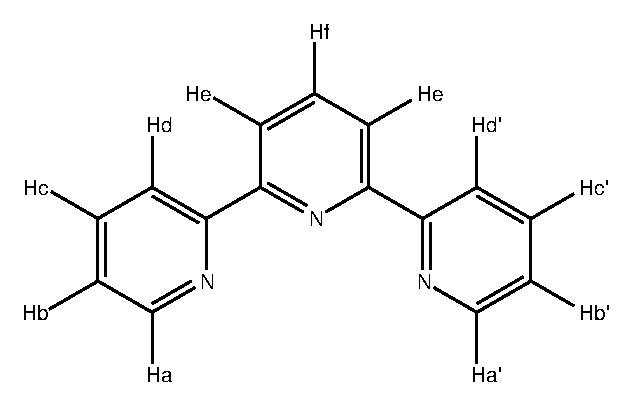
\includegraphics[clip=true, width=80mm, keepaspectratio]{images/expandedterpyridine.eps}
 \end{center}
\caption[Proton-explicit skeletal drawing of 2,2':6',2''-terpyridine]{Proton-explicit skeletal drawing of 2,2':6',2''-terpyridine}
\label{fig.terpynmr}
\end{figure} 

The simplification of peaks due to the symmetrization of the ligand results in the peaks from free pendant arm protons \textit{a}, \textit{b}, \textit{c}, and \textit{d} (see \autoref{fig.terpynmr}) with peaks at 9.06, 7.63, 8.22 and 7.79 ppm, respectively, aligning with their mirroring peaks at \textit{a'}, \textit{b'}, \textit{c'} and \textit{d'} (with peaks at 8.77, 7.55, 7.96, and 7.80 ppm). The new symmetrized peaks show integrations of two protons per peak, relative to the single proton (\textit{f}) peak from the central pyridyl ring, \textit{para} to the nitrogen. As well, the presence of metal-ligand interaction in the pendant arms reduces the deshielding effect, shifting the free pyridyl \textit{ortho} proton from 9.06 ppm to 8.77 in the chelated group, with similar shifts evident for the other pendant protons.

As in the case of bidentate compounds, modification of the anion has only minor effects on the \gls{ac.nmr} spectra. This is the expected behaviour, the conjugated pi system and the lack of protons near the modified anion combine to be susceptible in only a minor fashion.  

\begin{figure}[!htb]
 \begin{center}
  \includegraphics[clip=true, width=\textwidth, keepaspectratio]{images/allternmr.eps}
 \end{center}
\caption[The aromatic region of the \texorpdfstring{\ce{^1H}}{1H} \glsentrytext{ac.nmr} spectra of the four terdentate compounds]{The aromatic region of the \texorpdfstring{\ce{^1H}}{1H} \glsentrytext{ac.nmr} spectra for compounds \textbf{2.2} (blue), \textbf{2.4} (green), \textbf{2.6} (red) and \textbf{2.8} (purple)}
\label{fig.ter4nmr}
\end{figure} 

Carbon \gls{ac.nmr} (\ce{^{13}C}) was attempted on the complexes as well. Unfortunately, \ce{Re^I} complexes perform poorly in \ce{^{13}C}~\gls{ac.nmr} experiments, the signal to noise ratio is incredibly poor (if a signal is even visible). The effect of this is a lack of \ce{^{13}C} \gls{ac.nmr} analysis of these compounds in literature, with a very few exceptions. Extensive efforts included use of a 500 MHz spectrometer, with 1664 scans to produce the best example, seen in \autoref{fig.13cnmr}, with average peak signal to noise ratio (s/n) of only 4 - 5.

\begin{figure}[!htb]
 \begin{center}
  \includegraphics[clip=true, width=\textwidth, keepaspectratio]{images/13cnmr.eps}
 \end{center}
\caption[The 13C \glsentrytext{ac.nmr} spectra of \textbf{2.1}]{The \ce{^{13}C} \glsentrytext{ac.nmr} spectra of \textbf{2.1}. Spectra for other compounds could not be collected}
\label{fig.13cnmr}
\end{figure} 

\FloatBarrier

%----------------------------------------------------------------------
\subsection{Structure Analysis with X-Ray Crystallography and DFT}\label{ss.xray}
%----------------------------------------------------------------------

Single crystal analysis by x-ray crystallography yielded good structures of compounds \textbf{2.1}, \textbf{2.2}, \textbf{2.3}, \textbf{2.5}, and \textbf{2.8}. These are the first reported crystal structures of the $\kappa^3$~terdentate \ce{Re^I} compounds. A number of structural characteristics are common between the various bidentate or terdentate complexes. Much analysis has been done on the structures of bidentate complexes in literature\autocite{anderson1990, civitello1993, kurz2006} the notable characteristic within terpyridine compounds is the rotation of the pendant arm pushing the nitrogen atom away from the plane of the metal-ligand bonds by approximately 100$^\circ$. Cell parameters and other collection data for compounds \textbf{2.1}, \textbf{2.3}, \textbf{2.5}, and \textbf{2.7} are located in \autoref{tab.bidxraycp}.

% Table generated by Excel2LaTeX

\begin{table}[!htb]
  \caption{Crystal data and structure refinement for compounds \textbf{2.1}, \textbf{2.3}, and \textbf{2.5}}
  \resizebox{\textwidth}{!}{%
  \begin{tabular}{rp{3.2cm}p{3.2cm}p{3.2cm}}
    \toprule
    Compound & \textbf{2.1} & \textbf{2.3} & \textbf{2.5}  \\
    \cmidrule(l){2-4} 
    Empirical formula & \ce{C19H11N3O3ReCl} & \ce{C19H11N3O3ReBr} & \ce{C20H11N4O3Re} \\
    Formula weight (g/mol) & 538.96 & 583.41 & 530.04 \\
    Temperature (K) & 200 & 200 & 200 \\
    Wavelength (\r{A})  & 0.71073 & 0.71073 & 0.71073 \\
    Crystal System & Triclinic & Monoclinic & Triclinic \\
    Space Group & P-1 & C2/c & P-1  \\
    a (\r{A}) & 9.8736(4) & 31.1537(7) & 9.9196(9) \\
    b (\r{A}) & 14.8202(4) & 7.1176(2) & 14.9902(14) \\
    c (\r{A}) & 16.3472(4) & 16.8519(4) & 16.5187(15) \\
    $\alpha$ (deg) & 69.2890(10) & 90.000 & 68.363(2) \\
    $\beta$ (deg) & 80.801(2) & 111.0230(10) & 80.929(2) \\
    $\gamma$ (deg) & 79.836(2) & 90.000 & 79.975(2) \\
    Volume (\r{A}\textsuperscript{3}) & 2190.00(12) & 3488.00 & 2236.6(4) \\
    Z, r (calc) (Mg/m\textsuperscript{3}) & 2, 1.997 & 8, 2.222 & 2, 1.927 \\
    Absorption coefficient (mm\textsuperscript{-1}) & 6.063 & 9.282 & 5.821 \\
    Absorption correction  & \multicolumn{3}{c}{Semi-empirical from equivalents} \\
    Final R indices [I$\geq$2$\sigma$(I)] & R1 = 0.0397,\newline wR2 = 0.0839 & R1 = 0.0232,\newline wR2 = 0.0614 & R1 = 0.0390,\newline wR2 = 0.0921 \\
    R indices (all data) & R1 = 0.0604,\newline wR2 = 0.0951 & R1 = 0.0285,\newline wR2 = 0.0642 & R1 = 0.0500,\newline wR2 = 0.0961 \\
    \bottomrule
  \end{tabular}} 
  \label{tab.bidxraycp}%
\end{table}%



In addition, the structures of all species were optimized using Gaussian 09\autocite{gaussian} employing the B3LYP\autocite{becke1993, lee1988}  exchange-correlation (XC) functional. The LanL2DZ basis set/effective core potential\autocite{hay1985} was used on Re, and the all-electron TZVP basis set\autocite{schafer1994} for the remaining lighter atoms. Frequency analysis of all structures was used to confirm the nature of the stationary points. Solvent effects were computed when necessary using the integral equation formalism variant of the \gls{ac.pcm} for solvation within Gaussian 09\autocite{tomasi2005, scalmani2006}.The results of these calculations are compared to the x-ray crystallography data in the tables below.

The crystal structure of \textbf{2.3} had a higher symmetry than the other samples. Details on the exact methods used for structure elucidation are available in \autoref{sec.xray}, but all of the structures found are of high quality. The structures of \textbf{2.1}, \textbf{2.3}, and \textbf{2.5} can be seen in \autoref{fig.xraybid}. More views of these structures can be seen in Appendix \autoref{sec.xray}. Crystals suitable for x-ray analysis were unable to be collected from compound \textbf{2.7}. 

\begin{figure}[!ht]
 \centering
 \begin{subfigure}[b]{0.49\textwidth}
  \includegraphics[clip=true, width=\textwidth, keepaspectratio]{images/xray1a.eps}
  \caption{X-ray crystal structure for \textbf{2.1}}
  \label{fig.da1}
 \end{subfigure}
 \begin{subfigure}[b]{0.49\textwidth}
  \includegraphics[clip=true, width=\textwidth, keepaspectratio]{images/xray3a.eps}
  \caption{X-ray crystal structure for \textbf{2.3}}
  \label{fig.da3}
 \end{subfigure}
 \begin{subfigure}[b]{0.49\textwidth}
  \includegraphics[clip=true, width=\textwidth, keepaspectratio]{images/xray5a.eps}
  \caption{X-ray crystal structure for \textbf{2.5}}
  \label{fig.da5}
 \end{subfigure}
\caption[X-ray crystal structure representation for \textbf{2.1}, \textbf{2.3} and \textbf{2.5}.]{X-ray crystal structure representation for \textbf{2.1}, \textbf{2.3}, and \textbf{2.5}. Co-crystallized chloroform, hydrogen atoms, and thermal ellipsoids of ligand carbon atoms are omitted for clarity.}
\label{fig.xraybid}
\end{figure}

Selected bond lengths, bond angles, and torsion angles are listed in \autoref{tab.da1}, \autoref{tab.da3} and \autoref{tab.da5} for products \textbf{2.1}, \textbf{2.3}, and \textbf{2.5} respectively. The experimental results agree closely with the computed values for all samples. The structures can be seen in \autoref{fig.da1}, \autoref{fig.da3} and \autoref{fig.da5}, and more views of these structures can be seen in \autoref{chap.exp}, \autoref{ssec.views}, \nameref{ssec.views}. 

The \ce{Re^I} centre in the pseudooctahedral complex is supported by a planar, pincer coordinated ligand defined by the terminal and central pyridyl group of the terpyridine. One of the carbonyl groups lies in this plane trans to the central pyridyl group, while the remaining carbonyl groups and the anionic group or other complexed species lie on an approximately perpendicular plane to the ligand. Bond angles around the Re centre show a significant deviation of up to 15$^\circ$ from the ideal octahedral geometry for all samples analyzed. The typical N-Re-N bond angle of 75$^\circ$ is due to the atomic size of rhenium, comparison to the crystal structure of an analogous compound with a manganese atom\autocite{compain2014} shows an increase in the bonding angle for the \ce{Mn} complex by approximately 4$^\circ$ due to a decrease of bond length from metal to nitrogen of about 0.12~\r{A} for both the central and terminal pyridines. 

The deviation from octahedral is further visible in the rotation of the X-Re-CO plane (X=halide, anion, complexed group) by approximately 10 degrees from the right angle relative to the plane of the ligand. The axial halide, anion, or chelated group typically occupies a position slightly departed from the perpendicular, angled to be over the ligand. This eclipsing is due to some unknown process, no steric interference exists upon that site, analysis of electrostatic or other short-range electronic effects computationally show any interaction between this site and the aromatic rings. In \ce{Re^I} complexes, the halide or anion is located axial relative to the plane of the ligand. For the acetonitrile complex with triflate counterion, the acetonitrile occupies the axial position. This site occupation holds through the complete set of x-ray crystal structures with a \ce{$\kappa$^2-(bipy)Re(CO)3X} core structure motif deposited in the \gls{ac.ccdc} database\autocite{allen2002}, and extends through other $\alpha$-diimine complexes seen in our lab and in literature\autocite{jurca2013}. 

% Table generated by Excel2LaTeX
\begin{table}[!h]
\centering
 \begin{threeparttable}
  \caption{Solvated and gas phase energy differences between Axial \& Trans geometries of \ce{$\kappa$^x-(terpy)-Re(CO)_{5-x}CN} (x=2,3)}
    \begin{tabular}{cccc}
    \toprule
    \multicolumn{2}{c}{Bidentate} & \multicolumn{2}{c}{Terdentate} \\ \midrule
    E(gas)\tnote{a} & E(solution)\tnote{b} & E(gas)\tnote{a} & E(solution)\tnote{b} \\ \midrule
    14.70 & 11.87 & 16.28 & 16.43 \\
    \bottomrule
    \end{tabular}%
    \begin{tablenotes}
    \item [a] B3LYP SCF energy in kcal/mol.
    \item [b] B3LYP SCF energy in kcal/mol, with PCM solvation in acetonitrile.
    \end{tablenotes}
  \label{tab.cneng}%
 \end{threeparttable}
\end{table}%




The crystal structure for compound \textbf{2.5} contains two molecules per unit cell, one of which is solved to have the cyano group in the position trans to the ligand. However, careful analysis of the bond lengths, angles, and torsion data in \autoref{tab.da5} shows a remarked similarity between all -CO and -CN groups. Additionally, in an x-ray diffraction pattern, -CN and -CO are difficult to differentiate with certainty. Thus, while the structure solved to the two isomers, critical analysis would suggest that this molecule does not violate the axial position pattern laid out above. The computed structures energies in \autoref{tab.cneng} show a favouring of the axial position by 12-16 kJ/mol in the gas phase and by \gls{ac.pcm} in a simulated acetonitrile solvent. 

Selected bond lengths, bond angles, and torsions are listed in \autoref{tab.da1}, \autoref{tab.da3} and \autoref{tab.da5} for products \textbf{2.1}, \textbf{2.3}, and \textbf{2.5} respectively.

% Table generated by Excel2LaTeX
\begin{table}[htbp]
  \caption{Selected Distances, Angles, and Torsions for \textbf{1}}
  \centering
    \begin{tabular}{ccc}
    \toprule
    \multirow{2}{*}{Bond} & \multicolumn{2}{c}{Distance (\r{A})} \\ \cline{2-3}
     & Experimental & Calculated \\ \midrule
    Re(1)-C(16) & 1.89(1) & 1.916 \\
    Re(1)-C(17) & 1.934(8) & 1.936 \\
    Re(1)-C(18) & 1.90(1) & 1.918 \\
    Re(1)-N(1) & 2.162(6) & 2.197 \\
    Re(1)-N(2) & 2.236(9) & 2.293 \\
    Re(1)-Cl(1) & 2.496(2) & 2.525 \\ \midrule
    \multirow{2}{*}{Angle} & \multicolumn{2}{c}{Degrees ($^\circ$)} \\ \cline{2-3}
     & Experimental & Calculated \\ \midrule
    C(16)-Re(1)-C(17) & 87.6(4) & 86.877 \\
    C(16)-Re(1)-C(18) & 88.3(4) & 90.613 \\
    C(17)-Re(1)-C(18) & 87.3(4) & 89.557 \\
    C(16)-Re(1)-N(1) & 96.4(3) & 96.240 \\
    C(17)-Re(1)-N(1) & 174.9(3) & 175.600 \\
    C(18)-Re(1)-N(1) & 95.9(3) & 93.506 \\
    C(16)-Re(1)-N(2) & 169.3(3) & 170.368 \\
    C(17)-Re(1)-N(2) & 101.1(3) & 102.755 \\
    C(18)-Re(1)-N(2) & 98.3(3) & 89.415 \\
    N(2)-Re(1)-N(1) & 74.5(3) & 74.146 \\
    C(16)-Re(1)-Cl(1) & 91.7(3) & 91.453 \\
    C(17)-Re(1)-Cl(1) & 91.7(3) & 94.786 \\
    C(18)-Re(1)-Cl(1) & 179.9(3) & 175.286 \\
    N(1)-Re(1)-Cl(1) & 84.0(2) & 82.058 \\
    N(2)-Re(1)-Cl(1) & 81.6(2) & 87.840 \\
    O(1)-C(16)-Re(1) & 179.6(9) & 178.224 \\
    O(2)-C(17)-Re(1) & 176.0(8) & 176.907 \\ 
    O(3)-C(18)-Re(1) & 177.3(9) & 179.317 \\ \midrule
    \multirow{2}{*}{Torsion} & \multicolumn{2}{c}{Degrees ($^\circ$)} \\ \cline{2-3}
     & Experimental & Calculated \\ \midrule
    N(1)-C(5)-C(6)-N(2) &  16(1) & 15\\
    N(2)-C(10)-C(11)-N(3) & 41(1) & 139\\
    \bottomrule
    \end{tabular}%
  \label{tab.da1}%
\end{table}%



% Table generated by Excel2LaTeX
\begin{table}[htbp]
  \caption{Selected Distances, Angles, and Torsions for \textbf{2.3}}
  \centering
    \begin{tabular}{ccc}
    \toprule
   \multirow{2}{*}{Bond} & \multicolumn{2}{c}{Distance (\r{A})} \\ \cline{2-3}
     & Experimental & Calculated \\ \midrule
    Re(1)-C(16) & 1.911(3) & 1.91740 \\
    Re(1)-C(17) & 1.890(3) & 1.91814 \\
    Re(1)-C(18) & 1.921(4) & 1.93897 \\
    Re(1)-N(1) & 2.173(3) & 2.19687 \\
    Re(1)-N(2) & 2.232(2) & 2.28998 \\
    Re(1)-Br(1) & 2.6410(4) & 2.67953 \\ 
    C(16)-O(1) & 1.150(4) & 1.15290 \\
    C(17)-O(2) & 1.157(4) & 1.15012 \\
    C(18)-O(3) & 1.155(5) & 1.15591 \\ \midrule
    \multirow{2}{*}{Angle} & \multicolumn{2}{c}{Degrees ($^\circ$)} \\ \cline{2-3}
     & Experimental & Calculated \\ \midrule
    C(16)-Re(1)-C(17) & 89.1(1) & 90.772 \\
    C(16)-Re(1)-C(18) & 85.9(1) & 86.823 \\
    C(16)-Re(1)-N(1) & 97.9(1) & 96.034 \\
    C(17)-Re(1)-N(1) & 92.5(1) & 93.597 \\
    C(18)-Re(1)-N(1) & 175.4(1) & 175.575 \\
    C(16)-Re(1)-N(2) & 171.2(1) & 170.290 \\
    C(17)-Re(1)-N(2) & 96.0(1) & 89.435 \\
    C(18)-Re(1)-N(2) & 101.3(1) & 102.886 \\
    N(1)-Re(1)-N(2) & 74.7(1) & 74.265 \\
    C(16)-Re(1)-Br(1) & 92.7(1) & 90.399 \\
    C(17)-Re(1)-Br(1) & 177.6(1) & 176.076 \\
    C(18)-Re(1)-Br(1) & 91.6(1) & 94.069 \\
    N(1)-Re(1)-Br(1) & 85.74(7) & 82.555 \\
    N(2)-Re(1)-Br(1) & 82.07(7) & 88.780 \\
    O(1)-C(16)-Re(1) & 178.6(3) & 178.270 \\
    O(2)-C(17)-Re(1) & 179.5(3) & 179.355 \\
    O(3)-C(18)-Re(1) & 179.9(3) & 176.781 \\\midrule
    \multirow{2}{*}{Torsion} & \multicolumn{2}{c}{Degrees ($^\circ$)} \\ \cline{2-3}
     & Experimental & Calculated \\ \midrule
    N(1)-C(6)-C(1)-N(2) & -15.4(4) & -14.749 \\
    N(2)-C(5)-C(11)-N(3) & 141.1(3) & 136.119 \\
    \bottomrule
    \end{tabular}%
  \label{tab.da3}%
\end{table}%



% Table generated by Excel2LaTeX
\begin{table}[htbp]
  \caption{Selected Distances, Angles, and Torsions for \textbf{5}}
  \centering
    \begin{tabular}{cccc}
    \toprule
    \multicolumn{4}{c}{Selected Distances (\r{A})} \\ \midrule
    \multicolumn{2}{c}{Cyanide Axial} & \multicolumn{2}{c}{Cyanide Trans} \\ \midrule
    Re(2)-C(35) & 2.148(7) & Re(1)-C(19) & 2.105(8) \\
    Re(2)-C(36) & 1.926(6) & Re(1)-C(16) & 1.928(5) \\
    Re(2)-C(37) & 1.954(7) & Re(1)-C(18) & 1.96(1) \\
    Re(2)-C(38) & 1.902(9) & Re(1)-C(17) & 1.918(7) \\
    Re(2)-N(5) & 2.242(7) & Re(1)-N(1) & 2.253(5) \\
    Re(2)-N(6) & 2.168(5) & Re(1)-N(2) & 2.176(4) \\
    C(35)-N(8) & 1.138(9) & C(19)-O(3) & 1.17(1) \\
    C(36)-O(4) & 1.145(8) & C(16)-N(4) & 1.149(7) \\
    C(37)-O(5) & 1.151(9) & C(18)-O(2) & 1.14(1) \\
    C(38)-O(6) & 1.17(1) & C(17)-O(1) & 1.130(8) \\ \midrule
    \multicolumn{4}{c}{Selected Angles (deg)} \\ \midrule
    \multicolumn{2}{c}{Cyanide Axial} & \multicolumn{2}{c}{Cyanide Trans} \\ \midrule
    C(16)-Re(1)-C(17) & 87.8(3) & C(36)-Re(2)-C(38) & 87.7(3) \\
    C(16)-Re(1)-C(18) & 87.0(3) & C(36)-Re(2)-C(37) & 88.0(3) \\
    C(16)-Re(1)-C(19) & 92.5(3) & C(36)-Re(2)-C(35) & 92.1(3) \\
    C(17)-Re(1)-C(18) & 88.7(3) & C(38)-Re(2)-C(37) & 88.5(3)\\
    C(17)-Re(1)-C(19) & 90.5(3) & C(38)-Re(2)-C(35) & 90.8(3)\\
    C(18)-Re(1)-C(19) & 179.1(3) & C(37)-Re(2)-C(35) & 179.2(3) \\
    C(16)-Re(1)-N(1) & 102.2(2) & C(36)-Re(2)-N(5) & 100.6(3) \\
    C(16)-Re(1)-N(2) & 175.9(2) & C(36)-Re(2)-N(6) & 174.2(3) \\
    C(17)-Re(1)-N(1) & 168.3(3) & C(38)-Re(2)-N(5) & 169.3(3) \\
    C(17)-Re(1)-N(2) & 95.9(3) & C(38)-Re(2)-N(6) & 96.6(3) \\
    C(18)-Re(1)-N(1) & 97.7(3) & C(37)-Re(2)-N(5) & 98.4(2) \\
    C(18)-Re(1)-N(2) & 94.8(3) & C(37)-Re(2)-N(6) & 96.0(2) \\
    C(19)-Re(1)-N(1) & 83.2(2) & C(35)-Re(2)-N(5) & 82.3(2) \\
    C(19)-Re(1)-N(2) & 85.7(2) & C(35)-Re(2)-N(6) & 83.9(2) \\
    N(1)-Re(1)-N(2) & 73.9(2) & N(5)-Re(2)-N(6) & 74.7(2) \\
    O(1)-C(17)-Re(1) & 178.2(7) & O(6)-C(38)-Re(2) & 179.4(7) \\
    O(2)-C(18)-Re(1) & 172.0(7)& O(5)-C(37)-Re(2) & 175.5(6) \\ 
    O(3)-C(19)-Re(1) & 178.0(6) & N(8)-C(35)-Re(2) & 178.0(6) \\
    N(4)-C(16)-Re(1) & 178.7(6) & O(4)-C(36)-Re(2) & 179.0(7) \\ \midrule
    \multicolumn{4}{c}{Selected Torsions (deg)} \\ \midrule
    \multicolumn{2}{c}{Cyanide Axial} & \multicolumn{2}{c}{Cyanide Trans} \\ \midrule
    N(1)-C(1)-C(6)-N(2) & 12.5(8) & N(5)-C(20)-C(25)-N(6) & 14.5(9) \\
    N(1)-C(5)-C(11)-N(3) & 43.7(9) & N(5)-C(24)-C(30)-N(7) & 41(1) \\
    \bottomrule
    \end{tabular}%
  \label{tab.da5}%
\end{table}%




\FloatBarrier

Structural comparisons between the bidentate samples and the terdentate show many similarities. The loss of one carbonyl always accompanies the chelation of the pendant arm of the ligand. The increased coordination forces the ligand to adopt a more rigidly planar geometry, this is visible in the structure of \textbf{2.2} (\autoref{fig.da2}) and \textbf{2.8} (\autoref{fig.da8}). Suitable crystals for x-ray analysis were unable to be collected for the remaining complexes.

\begin{figure}[!ht]
 \centering
 \begin{subfigure}[b]{0.49\textwidth}
  \includegraphics[clip=true, width=\textwidth, keepaspectratio]{images/xray2a.eps}
  \caption{X-ray crystal structure for \textbf{2.2}}
  \label{fig.da2}
 \end{subfigure}
 \begin{subfigure}[b]{0.49\textwidth}
  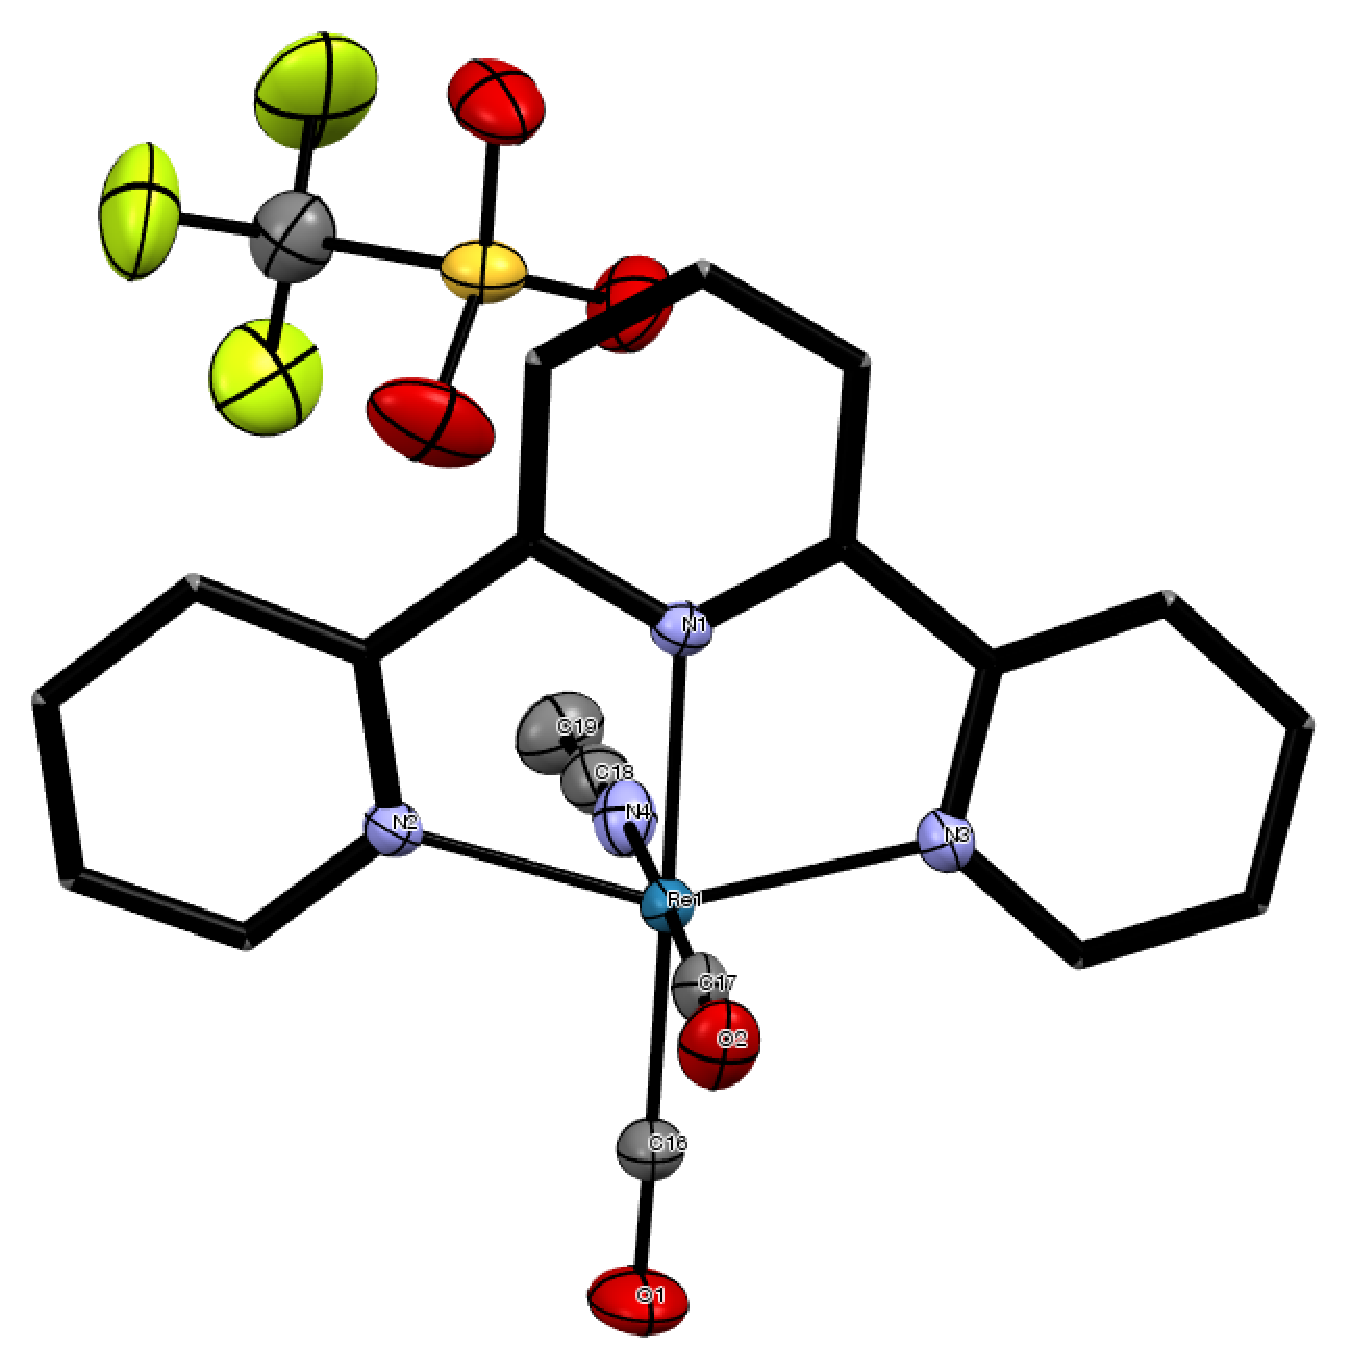
\includegraphics[clip=true, width=\textwidth, keepaspectratio]{images/xray8a.eps}
  \caption{X-ray crystal structure for \textbf{2.8}}
  \label{fig.da8}
 \end{subfigure}
\caption[X-ray crystal structure representation for \textbf{2} and \textbf{8}.]{X-ray crystal structure representation for \textbf{2.2} and \textbf{2.8}. Co-crystallized chloroform, hydrogen atoms, and thermal ellipsoids of ligand carbon atoms are omitted for clarity.}
\label{fig.xrayter}
\end{figure} 

Selected bond lengths, bond angles, and torsions are listed in \autoref{tab.da2} and \autoref{tab.da8} for products \textbf{2.2} and \textbf{2.8}. Cell parameters and collection data can be found in \autoref{tab.terxraycp}. 

Both \textbf{2.2} and \textbf{2.8} structures are pseudooctahedral in geometry, with \textit{mer} coordinated terpyridine ligand. The carbonyl groups and chloride/acetonitrile form a plane approximately perpendicular to the ligand. As in the \ce{$\kappa$^2}-bidentate samples discussed above, the carbonyls occupy the equatorial and one axial position relative to the ligand, and the chloride or acetonitrile occupy the remaining axial position. The N-Re-N bond angles remain approximately 75$^\circ$, and the central pyridyl N to chloride or acetonitrile angle is still approximately 80-85$^\circ$. 

Comparisons between the \ce{$\kappa$^2}-bidentate and \ce{$\kappa$^3}-terdentate samples (\textbf{2.1} and \textbf{2.2}) highlight the geometrical changes experienced in the thermolysis reaction. The distance from Re to the central pyridyl N has shortened from 2.24~to~2.08~\r{A}. This bond shortening of 0.16~\r{A} signifies increased metal-ligand interaction. This comes at the expense of decreased interaction with the carbonyl groups, with the bond to the planar \ce{CO} increasing from 1.89 to 1.93~\r{A} and the axial \ce{CO} bond increasing from 1.901 to 1.975~\r{A}. As the carbonyls experience less $\pi$ backbonding from the metal, the internal C-O bond shortens by as much as 0.1~\r{A}. 

The \ce{$\kappa$^3}-terdentate samples (\textbf{2.2} and \textbf{2.8}) provide the opportunity to analyze both neutral and cationic species. Due to the weakly coordinated triflate anion in \textbf{2.8}, a number of geometric differences arise compared to \textbf{2.2}. While the ligand is coordinated by only 0.01 - 0.02~\r{A} closer to the metal atom, the carbonyl groups are 0.04 - 0.1~\r{A} closer, indicating their increased electron donation to the electron poor metal centre. As well, the C-O bonds in the carbonyls are 0.03 - 0.12~\r{A} longer, indicating the increased $\pi$-backbonding occurring in the cation.  

% Table generated by Excel2LaTeX
\begin{table}[htbp]
  \caption{Selected Distances, Angles, and Torsions for \textbf{2.2}}
  \centering
    \begin{tabular}{ccc}
    \toprule
    \multirow{2}{*}{Bond} & \multicolumn{2}{c}{Distance (\r{A})} \\ \cline{2-3}
     & Experimental & Calculated \\ \midrule
    Re(1)-C(16) & 1.926(9) & 1.92438\\
    Re(1)-C(17) & 1.975(10) & 1.90687\\
    Re(1)-N(1) & 2.119(7) & 2.13186\\
    Re(1)-N(2) & 2.080(7) & 2.08705\\
    Re(1)-N(3) & 2.126(7) & 2.13185\\
    Re(1)-Cl(1) & 2.489(3) & 2.53337 \\
    N(1)-N(3) & 4.14(1) & 4.14772 \\ 
    C(16)-O(1) & 1.14(1) & 1.16042 \\
    C(17)-O(2) & 1.05(1) & 1.16341 \\ \midrule
    \multirow{2}{*}{Angle} & \multicolumn{2}{c}{Degrees ($^\circ$)} \\ \cline{2-3}
     & Experimental & Calculated \\ \midrule
    C(16)-Re(1)-C(17) & 91.5(4) & 89.188 \\
    C(16)-Re(1)-N(2) & 173.7(4) & 172.050 \\
    C(17)-Re(1)-N(2) & 94.6(3) & 98.762 \\
    C(16)-Re(1)-N(1) & 103.9(3) & 102.980 \\
    C(17)-Re(1)-N(1) & 92.7(3) & 93.429 \\
    N(2)-Re(1)-N(1) & 77.3(3) & 76.684 \\
    C(16)-Re(1)-N(3) & 101.8(3) & 102.986 \\
    C(17)-Re(1)-N(3) & 91.7(3) & 93.419 \\
    N(2)-Re(1)-N(3) & 76.6(3) & 76.684 \\
    N(1)-Re(1)-N(3) & 153.7(3) & 153.210 \\
    C(16)-Re(1)-Cl(1) & 91.8(3) & 89.136 \\
    C(17)-Re(1)-Cl(1) & 176.5(2) & 178.324 \\
    N(2)-Re(1)-Cl(1) & 82.1(2) & 82.913 \\
    N(1)-Re(1)-Cl(1) & 85.4(2) & 86.953 \\
    N(3)-Re(1)-Cl(1) & 88.7(2) & 86.953 \\
    O(1)-C(16)-Re(1) & 177.9(9) & 179.079 \\
    O(2)-C(17)-Re(1) & 173.2(8) & 179.182 \\ \midrule
    \multicolumn{2}{c}{Selected Torsions (deg)} \\ \midrule
    N(1)-C(5)-C(6)-N(2) & 1(1) & 2 \\
    N(2)-C(10)-C(11)-N(3) & -4(1) & -2 \\
    \bottomrule
    \end{tabular}%
  \label{tab.da2}%
\end{table}%



% Table generated by Excel2LaTeX from sheet 'Sheet3'
\begin{table}[htbp]
  \centering
  \caption{Selected Distances, Angles and Torsions for Acetonitrile Adduct of \textbf{2.8}}
    \begin{tabular}{ccc}
    \toprule
	\multirow{2}{*}{Bond} & \multicolumn{2}{c}{Distance (\r{A})} \\ \cline{2-3}
     & Experimental & Calculated \\ \midrule
    Re(1)-C(16) & 1.889(4) & 1.93046 \\
    Re(1)-C(17) & 1.885(3) & 1.92844 \\
    Re(1)-N(1) & 2.091(3) & 2.10116 \\
    Re(1)-N(2) & 2.135(3) & 2.15397 \\
    Re(1)-N(3) & 2.131(3) & 2.15392 \\
    Re(1)-N(4) & 2.160(3) & 2.15202 \\ 
    N(2)-N(3) & 4.138(4) & 4.18483 \\ 
    C(16)-O(1) & 1.170(4) & 1.15749 \\
    C(17)-O(2) & 1.171(4) & 1.15244 \\ \midrule
	\multirow{2}{*}{Angle} & \multicolumn{2}{c}{Degrees ($^\circ$)} \\ \cline{2-3}
     & Experimental & Calculated \\ \midrule
    C(16)-Re(1)-C(17) & 87.69(16) & 88.104 \\
    C(16)-Re(1)-N(1) & 175.95(12) & 176.094 \\
    C(17)-Re(1)-N(1) & 96.35(12) & 95.802 \\
    C(16)-Re(1)-N(3) & 103.81(13) & 103.594 \\
    C(17)-Re(1)-N(3) & 94.03(12) & 92.309 \\
    N(1)-Re(1)-N(3) & 76.20(10) & 76.306 \\
    C(16)-Re(1)-N(2) & 103.58(13) & 103.598 \\
    C(17)-Re(1)-N(2) & 93.73(12) & 92.307 \\
    N(1)-Re(1)-N(2) & 75.99(10) & 76.305 \\
    N(3)-Re(1)-N(2) & 151.77(11) & 152.544 \\
    C(16)-Re(1)-N(4) & 90.50(14) & 88.484 \\
    C(17)-Re(1)-N(4) & 178.10(12) & 176.587 \\
    N(1)-Re(1)-N(4) & 85.46(10) & 87.611 \\
    N(3)-Re(1)-N(4) & 86.94(10) & 88.504 \\
    N(2)-Re(1)-N(4) & 86.15(10) & 88.485 \\
    O(1)-C(16)-Re(1) & 179.1(3) & 178.807 \\
    O(2)-C(17)-Re(1) & 178.0(3) & 178.860 \\\midrule
    \multirow{2}{*}{Torsion} & \multicolumn{2}{c}{Degrees ($^\circ$)} \\ \cline{2-3}
     & Experimental & Calculated \\ \midrule
    N(1)-C(1)-C(6)-N(2) & 1.7(4) & 1.105 \\
    N(1)-C(5)-C(11)-N(3) & -1.8(4) & -1.110 \\
    \bottomrule
    \end{tabular}%
  \label{tab.da8}%
\end{table}%

% Table generated by Excel2LaTeX
\begin{table}[!htb]
\centering
  \caption{Crystal data and structure refinement for compounds \textbf{2.2} and \textbf{2.8}}
    \begin{tabular}{rp{3.2cm}p{3.2cm}}
    \toprule
    Compound & \textbf{2.2} & \textbf{2.8} \\
    \cmidrule(l){2-3} 
    Empirical formula& \ce{C18H11N3O2ReCl} & \ce{C21H14N4O5F3SRe} \\
    Formula weight (g/mol) & 510.95 & 665.61 \\
    Temperature (K) & 200 & 200 \\
    Wavelength (\r{A}) & 0.71073 & 0.71073 \\
    Crystal System & Triclinic & Triclinic \\
    Space Group & P-1 & P-1 \\
    a (\r{A}) & 8.5275(3) & 8.5745(4) \\
    b (\r{A}) & 14.2421(5) & 11.9805(5) \\
    c (\r{A}) & 17.4637(6) & 13.0970(5) \\
    $\alpha$ (deg) & 77.948(2) & 79.748(2) \\
    $\beta$ (deg) & 85.684(2) & 81.106(2) \\
    $\gamma$ (deg) & 79.890 & 88.091(2) \\
    Volume (\r{A}\textsuperscript{3}) & 2041.79(12) & 1307.99(10) \\
    Z, r (calc) (Mg/m\textsuperscript{3}) & 4, 2.050 & 2, 1.993 \\
    Absorption coefficient (mm\textsuperscript{-1}) & 6.494 & 5.094 \\
    Absorption correction  & \multicolumn{2}{c}{Semi-empirical from equivalents} \\
    Final R indices [I$\geq$2$\sigma$(I)] & R1 = 0.0636,\newline wR2 = 0.1018 & R1 = 0.0294,\newline wR2 = 0.0673 \\
    R indices (all data) & R1 = 0.0985,\newline wR2 = 0.1110 & R1 = 0.0366,\newline wR2 = 0.0700 \\
    \bottomrule
    \end{tabular}%
  \label{tab.tercellparams}%
\end{table}%

\FloatBarrier

%----------------------------------------------------------------------
\subsection{Infrared Spectroscopy}
%----------------------------------------------------------------------

Conversion of bidenate to terdentate species was confirmed utilizing \gls{ac.ftir} spectroscopy. A small sample of powder product was placed on the Agilent Cary 630 \gls{ac.ftir} spectrometer, with a 2 \ce{cm^{-1}} resolution. The instrument is fitted with a diamond ATR for solid sample analysis. Spectra are the Fourier transform of 16 scans.

\begin{figure}[!htb]
 \begin{center}
  \includegraphics[clip=true, width=\textwidth]{images/ftir1and2.eps}
 \end{center}
\caption[FTIR Spectra for complexes \textbf{2.1} and \textbf{2.2}]{FTIR Spectra for complexes \textbf{2.1} (blue) and \textbf{2.2} (red).}
\label{fig.ir1}
\end{figure} 

Analysis of the results in \autoref{fig.ir1} shows the significant reduction of one peak in the (ca.) 2100 \ce{cm^{-1}} region. This peak is in the CO stretching frequency, the frequency of the peak lost in thermolysis is indicative of a weakly coordinated carbonyl group. A splitting occurs for the other large peak and its shoulder in the conversion from bidentate to terdentate, from 1890 to 1790 \ce{cm^{-1}}, indicating the further weakening of the metal carbonyl bonds remaining in the complex. This weakened bond is likely the carbonyl co-planar to the ligand, analysis of the x-ray crystal structure shows the CO bond to be 0.1~\r{A} longer than that of the axial carbonyl. This identification is supported by the \gls{ac.dft} methods discussed below.

\begin{figure}[!htb]
 \centering
 \includegraphics[clip=true, width=\textwidth, keepaspectratio]{images/ftircomputational.eps}
 \caption[DFT predicted FTIR spectra for \textbf{2.1} and \textbf{2.2}]{DFT predicted FTIR spectra for \textbf{2.1} (blue) and \textbf{2.2} (red).}
 \label{fig.ircomp}
\end{figure}

\Gls{ac.ftir} spectra were predicted using molecular frequency calculations of \gls{ac.dft} optimized structures in Gaussian09. Prediction of this spectra was performed as a verification of the optimized structures discussed in \autoref{ss.xray} above. The calculation identifies stretching or bending harmonic energies in optimized structures. The computed spectra in \autoref{fig.ircomputed} shows three peaks for \textbf{2.1}, at 2094, 2012, and 1990 \ce{cm^{-1}}. The relative location of these peaks corresponds to those seen in \autoref{fig.ircomp} for \textbf{2.1}, but are shifted by approximately 100 \ce{cm^{-1}} to higher energy relative to the experimental. Similarly, for \textbf{2.2}, peaks are seen at 2000 and 1950 \ce{cm^{-1}}, compared to the 1890 and 1790 peaks seen experimentally. This computed value reflects the shift to lower energy carbonyl stretching from \textbf{2.1} to \textbf{2.2}, and echoes the experimental spectra well.

Further analysis of other spectra were not successful in identification of any additional molecular properties, with the exception of a series of strong peaks appearing in the 1200-1300 \ce{cm^{-1}} range, confirming the presence of the triflate anion from the -\ce{SO3} group vibrations for samples \textbf{2.7} and \textbf{2.8} (\autoref{fig.ir78}). Additionally, the small peak present at 2270 \ce{cm^{-1}} in the terdentate sample corresponds to the weakly coordinated acetonitrile occupying the moluecule's axial position.

\begin{figure}[!htb]
 \centering
 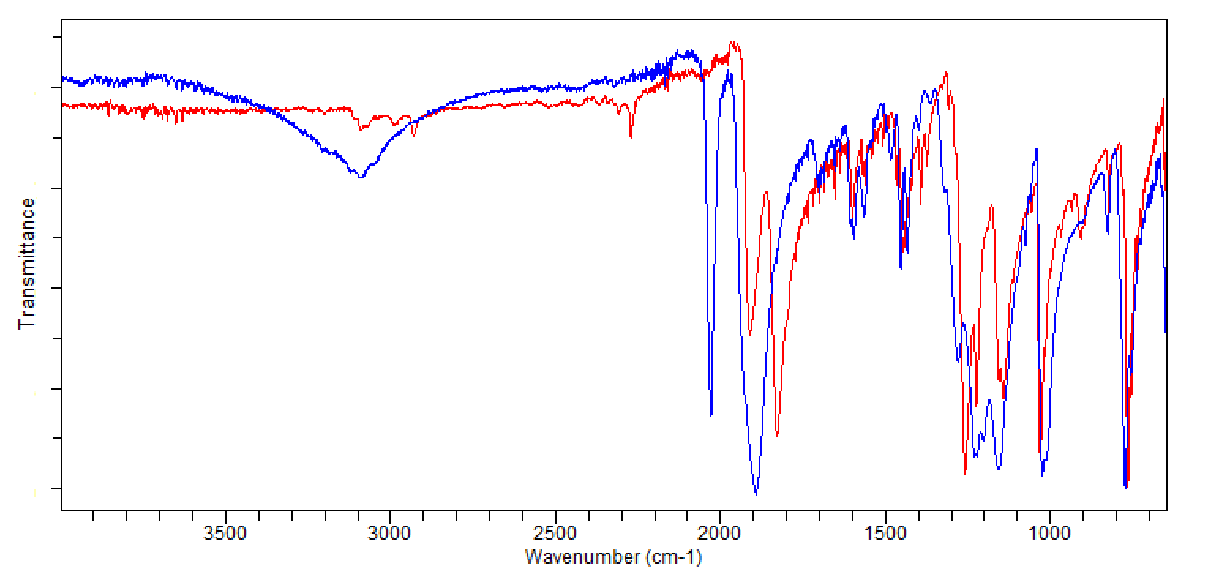
\includegraphics[clip=true, width=\textwidth, keepaspectratio]{images/ftir7and8.eps}
 \caption[FTIR Spectra for complexes \textbf{2.7} and \textbf{2.8}]{FTIR Spectra for complexes \textbf{2.7} (blue) and \textbf{2.8} (red).}
 \label{fig.ir78}
\end{figure}

\FloatBarrier
%----------------------------------------------------------------------
\subsection{Photophysical Properties}
%----------------------------------------------------------------------

A striking observation upon the conversion of the bidentate species into the terdentate complexes is that these new compounds have a substantially darker colour that reflects a significant change in the photophysical properties. This effect was investigated using a combination of UV-visible spectroscopy and \gls{ac.dft} modelling. Spectra were collected on a Agilent Cary 5000 UV-Vis-NIR Spectrophotometer. The stronger absorbance of the terdentate complexes compared to the bidentate precoursors is evident in the UV-Vis spectra of these species, and is presented in \autoref{fig.uvvisexps}. These spectra were obtained in \gls{ac.dmso} with approximate concetrations of 0.01 mM for bidentate, and an order of magnitude lower (0.001 mM) for the terdentate analogues. The terdentate complexes have more intense absorbance for higher energy ligand UV-based $\pi$-$\pi^\ast$ transitions (\textless 400 nm) and certainly a richer visible absorption profile that involve the d-$\pi^\ast$ transitions. These features are responsible for the colour change observed.

\begin{figure}[!htb]
 \centering
 \begin{subfigure}[b]{0.49\textwidth}
  \includegraphics[clip=true, width=\textwidth]{images/bidentateuvvis.eps}
  \caption{UV-Vis spectra for compounds \textbf{2.1}, \textbf{2.3}, \textbf{2.5}, and \textbf{2.7}}
  \label{fig.uvvisbids}
 \end{subfigure}
 \begin{subfigure}[b]{0.49\textwidth}
  \includegraphics[clip=true, width=\textwidth]{images/terdentateuvvis.eps}
  \caption{UV-Vis spectra for compounds \textbf{2.2}, \textbf{2.4}, \textbf{2.6}, and \textbf{2.8}}
  \label{fig.uvvisters}
 \end{subfigure}
\caption[UV-Vis spectra for all compounds]{UV-Vis spectra for all compounds. Concentrations of bidentate complexes are 0.01 mM and terdentate complexes are 0.001 mM.}
\label{fig.uvvisexps}
\end{figure} 

The UV-Vis spectra were modeled using \gls{ac.tddft} computations within Gaussian 09, using the B3LYP functional with the LanL2DZ basis set and effective core potentials for the rhenium atom, and the TZVP basis set for all lighter atoms. Such functional and basis set choices are common within organometallic literature. Solvent was simulated using the integral equation formalizm variant of the \gls{ac.pcm} solvation model, with DMSO as the solvent. 

The resulting computed spectra were excellent matches to the experimental spectra. The similarity of the spectra between the bidentate species and as well as the terdentate species indicates that parallel electronic transitions appear within these two groups. Specifics will be discussed for the chloro compounds, \textbf{2.1} and \textbf{2.2}, but strong parallels exist for all species. Plots of experimental and computational data for these two complexes are presented in \autoref{fig.uvvisbidec} and \autoref{fig.uvvisterec}, respectively.

\begin{figure}[!htb]
 \centering
  \includegraphics[clip=true, width=120mm, height=120mm, keepaspectratio]{images/uvvisbidec.eps}
 \caption[Plots of the experimental and computed UV-Vis spectra for compound \textbf{2.1}]{Plots of the experimental and computed UV-Vis spectra for compound \textbf{2.1}. The blue curve shows experimental result.The red vertical lines show the calculated transitions and relative intensities from the TDDFT calculations, while the red curve shows the Gauss convolution with peak width at half height of 0.250 eV.}
 \label{fig.uvvisbidec}
\end{figure}

\begin{figure}[!htb]
 \centering
  \includegraphics[clip=true, width=120mm, height=120mm, keepaspectratio]{images/uvvisterec.eps}
 \caption[Plots of the experimental and computed UV-Vis spectra for compound \textbf{2.2}]{Plots of the experimental and computed UV-Vis spectra for compound \textbf{2.2}.  The blue curve shows experimental result.The red vertical lines show the calculated transitions and relative intensities from the TDDFT calculations, while the red curve shows the Gauss convolution with peak width at half height of 0.250 eV.}
 \label{fig.uvvisterec}
\end{figure}

Common to all bidentate compounds were peaks at wavelengths of 315-320 nm, and peak shoulders near 350-375 nm (\autoref{fig.uvvisbids}). In the case of \textbf{2.1}, the computational results suggest that the experimental band centred at $\lambda$ = 315-320 nm (31750-31250 \ce{cm^{-1}}) primarily arises from two electronic transitions. The first is from HOMO-3 to LUMO, a $\pi$-$\pi^\ast$ transition, while the second major contribution is the excitation from HOMO to LUMO+2, which is a d-$\pi^\ast$ transition. The \gls{ac.tddft} calculations suggest that the experimental band centred at $\lambda$ = 370 nm (27030 \ce{cm^{-1}}) corresponds to a calculated transition at approximately 400 nm, that is a d-$\pi^\ast$ (HOMO-1 to LUMO) absorbance. Computed plots of molecular orbitals are included in \autoref{app.mos} \nameref{app.mos}, \Cref{fig.mo21,fig.mo22,fig.mo23,fig.mo24,fig.mo25,fig.mo26,fig.mo27,fig.mo28}.

Like the bidentate samples, the spectra for the terdentate samples are quite similar to one another. In general, all of these species have much higher absorbance coefficients than their bidentate analogues; all contain long trailing absorptions across the wavelengths analysed. For terdentate complex \textbf{2.2}, the four experimentally observed UV-Vis absorptions observed are made up of six computed transitions. The computational model provided two equal and strong tranitions appearing at 308 and 325 nm to generate the experimental band centred at $\lambda$ = 330 nm (30300 \ce{cm^{-1}}). These arise from a transition from HOMO-5, to LUMO, a Cl lone-pair to terpy $\pi^\ast$-orbital absorption, and from HOMO-3 to LUMO, which is a ligand centred $\pi$-$\pi^\ast$ transition. All of the lower energy transitions are dominated by MLCT bands. The experimental band centered at $\lambda$ = 400 nm (25000 \ce{cm^{-1}}) arises from an electronic transition from HOMO to LUMO+3 which is d-$\pi^\ast$ in nature. The absorbance centred at $\lambda$ = 460 nm (21740 \ce{cm^{-1}}) corresponds to two MLCT d-$\pi^\ast$ transitions; HOMO-2 to LUMO and HOMO-1 to LUMO+1. Finally, the broad experimental band 680-715 nm (14700-14000 \ce{cm^{-1}}) arises from the electronic transition appearing at 718 nm, which is the excitation of a d-electron in the Re-centered HOMO to the ligand $\pi^\ast$ LUMO.

\FloatBarrier
%----------------------------------------------------------------------
\subsection{Fluorescence}\label{ss.fluorescence}
%----------------------------------------------------------------------

Fluorescence data was collected for \textbf{2.1} and \textbf{2.2} using an Agilent Cary Eclipse Fluorescence Spectrophotometer, using a 5 nm excitation slit and emission slit, using excitation wavelengths selected to correspond to the centre of UV-Vis absorption bands. Data was collected for spectra in \gls{ac.dmf} to simulate the photocatalytic reaction environment (see \autoref{chap.co2}). Spectra are shown in \autoref{fig.fluoro} for \textbf{2.1} and \textbf{2.2} with their UV-Vis absorption spectra for comparison. Data is normalized to equil concentration for each sample in fluorescence and absorbance.

\begin{figure}[!htb]
 \centering
  \includegraphics[clip=true, width=140mm, height=100mm, keepaspectratio]{images/fluoro.eps}
 \caption[UV-Vis and fluorescence spectra for \textbf{2.1} and \textbf{2.2}]{UV-Vis and fluorescence spectra for \textbf{2.1} and \textbf{2.2}. Fluorescence of \textbf{2.1} from excitation of 373 nm (blue), excitation of \textbf{2.2} by 400 nm (red) and 470 nm (green) are shown, along with the absorption spectra of \textbf{2.1} (purple) and \textbf{2.2} (orange).}
 \label{fig.fluoro}
\end{figure}

Clearly the transformation from bidentate terpyridine to terdentate ligand has significant effect on the interactions of these Re compounds with visible light. Terdentate samples fluoresce and absorb more intensely at lower energy wavelengths. While the terdentate sample is excited at various wavelengths (that should correspond to different absorption bands), the emission appears to be from one single band centred at ca. 490 nm. 

Interestingly, emission is not seen with the naked eye with 400 nm excitation for the terdentate, while the bidentate emission is very strong. This may be due to self-absorbance in the terdentate samples, emission of 490 nm is easily absorbed by the molecule. In the bidentate, no absorbance bands correspond with emission seen at 470 nm or 600 nm, these appear to the naked eye as a white emission.

\FloatBarrier
%----------------------------------------------------------------------
\section{Conclusions}
%----------------------------------------------------------------------

This work reported the first crystallographically authenticated rhenium(I) terpyridine terdentate complexes and thus expanded upon the prior limitations of Re coordination complexes. These terpyridine complexes are accessed via a simple, highly efficient, solid-state thermolysis pathway. They expand upon the known $\alpha$-diimine photophysical properties, with enhanced metal-to-ligand d-$\pi^\ast$ electronic transitions, occurring more frequently and with lower energy than in the associated bidentate compounds. These observations are supported by computational \gls{ac.tddft} results, affording an expanded understanding of the transition bands. Modification of the bidentate and terdentate species has been shown, the synthetic success of a triflate moiety should facilitate further development of reactivity and provides an opportunity for synthetic and catalytic studies.



